%
% Appendix B
%

\chapter{Misidentification rate method}
\label{fakefactor}

The misidentified lepton background is dominant in hadronic channels, and it is estimated using the misidentification rate method discussed in Chapter~\ref{bkg_est}. The systematic uncertainties associated with estimating the misidentified lepton background impact the median expected limits significantly. To recap, we are using a normalization uncertainty of 30\% for the misidentified lepton background along with a 10\% normalization uncertainty uncorrelated across the categories of each channel. Similarly, the shape uncertainties are estimated in a \PW boson enriched control region, and these uncertainties have a high impact and are constrained by the data. To improve the analysis's sensitivity, we need a better handle on the misidentified lepton background and its associated uncertainties. An improvement to the misidentification rate method is presented here.

Since the jet flavor composition of different background processes is different, leading to different probabilities of these jets getting misidentified as \tauh, the misidentification rate is measured separately for each dominant process. The dominant background processes are \wjets, QCD multijet, and \ttbar. First, determination regions are defined, each enriched in one of the above backgrounds. From each determination region, one extracts a dedicated misidentification rate, which is parametrized by its main dependencies to reduce statistical fluctuation. Further, so-called closure corrections in important variables not used in the misidentification rates parametrization are calculated. Contaminations in the different determination regions other than the process of interest are subtracted from data by using MC simulation and embedding samples. The misidentification rate is applied on an event-by-event basis as a weighted sum in the so-called application region. The application region is equivalent to the ``background-like'' region and signal region is equivalent to the ``signal-like'' region defined in Chapter~\ref{bkg_est}. The weights applied to each misidentification rate contribution are called fractions and represent the probability of the event being of a particular background process. Fractions are determined from MC simulation and embedding samples. Figure~\ref{fig:ff} shows a graphical summary of the misidentification rate method.

\begin{figure}[htbp]
  \centering
  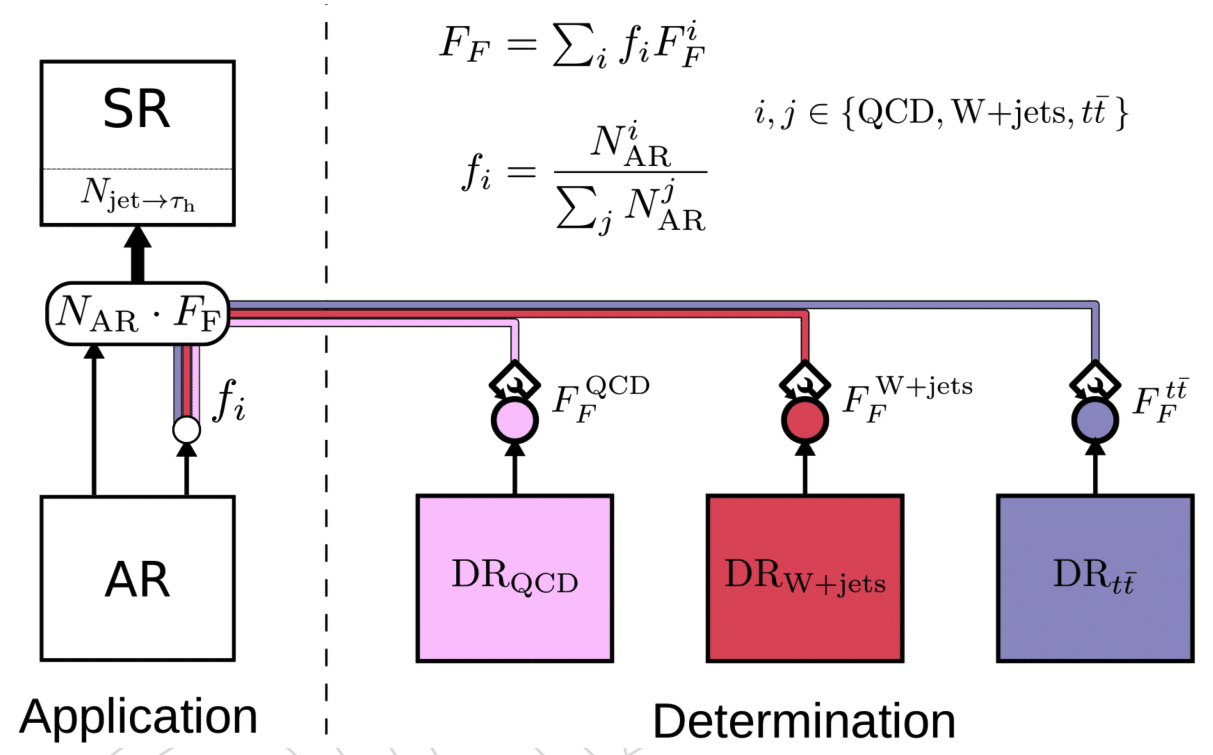
\includegraphics[width=0.9\textwidth]{plots/appendix/FF.png}
  \caption{Illustration of the misidentification rate method. For each of the processes (\wjets, QCD, and \ttbar), a dedicated misidentification rate is measured in a process enriched determination region. The measured misidentification rate is corrected and then applied on an event by event basis inside the application region. The application of the misidentification rate inside the application region also involves the fractions $f_i$, representing the probabilities of an event in the application region originating from process $i$.}
  \label{fig:ff}
\end{figure}

The basic assumption of the misidentification rate method is the so-called universality. The misidentification rate measured in a determination region is the same as if measured in the signal region or any other phase space region. Universality is not strictly given because by measuring the misidentification rate in a determination region, one introduces biases—for example, the jet-flavor composition changes in the determination region with respect to the signal region. Therefore, the misidentification rate method also implements process-dependent bias corrections to restore the misidentification rate universality. In summary, the misidentification rate is measured in dedicated determination regions and parametrized in variables reflecting its most dominant dependencies. Afterward, corrections are derived for improving the modeling of the jet-\tauh misidentified contribution in variables not used for the parametrization. A last step bias correction is calculated, accounting for possible differences between the determination region where the misidentification rate is measured and the application region where the misidentification rate is applied.

A future Higgs boson LFV decays search can benefit from using this method for calculating the misidentified lepton background in hadronic channels. The corrections used for improving the modeling and the bias corrections can give a better description of the misidentified lepton background in hadronic channels. This method has been successfully incorporated in the SM \Htt analyses~\cite{CMS:2019pyn}.
